\documentclass[11pt]{article}
% =============================================================================
% preamble.tex — shared LaTeX preamble for the Pagesmith guides.
% \input this from each guide's .tex. Verified to compile with pdflatex (TeX Live).
% =============================================================================
\usepackage[margin=1in]{geometry}
\usepackage{amsmath,amssymb}
\usepackage{microtype}
\usepackage{enumitem}
\usepackage{xcolor}
\usepackage{hyperref}
\usepackage{listings}
\usepackage{tikz}
\usetikzlibrary{positioning,arrows.meta,shapes.geometric,calc,fit,backgrounds}
\usepackage{placeins}   % \FloatBarrier
\usepackage{caption}
\captionsetup{font=small,skip=8pt}

\hypersetup{colorlinks=true,linkcolor=blue!55!black,urlcolor=blue!55!black,citecolor=blue!55!black}

% A bit of breathing room around floats.
\setlength{\textfloatsep}{16pt plus 4pt minus 4pt}
\setlength{\intextsep}{16pt plus 4pt minus 4pt}

% ---- code listings ----------------------------------------------------------
\definecolor{codebg}{RGB}{248,248,248}
\definecolor{codecmt}{RGB}{0,128,0}
\definecolor{codestr}{RGB}{170,55,0}
\definecolor{codekw}{RGB}{0,0,180}
% No fixed `language=` (so neither JS nor JSON trips listings' keyword parser);
% code is shown as clean monospace in a framed, tinted box.
\lstset{
  basicstyle=\ttfamily\small,
  backgroundcolor=\color{codebg},
  commentstyle=\color{codecmt}\itshape,
  stringstyle=\color{codestr},
  showstringspaces=false,
  breaklines=true,
  columns=fullflexible,
  keepspaces=true,
  frame=single,
  framesep=4pt,
  rulecolor=\color{black!20},
  aboveskip=10pt,
  belowskip=6pt
}

% ---- tikz diagram helpers (boxes + arrows) ----------------------------------
\definecolor{boxblue}{RGB}{79,124,255}
\definecolor{boxgray}{RGB}{90,98,112}
\tikzset{
  box/.style   = {draw, rounded corners, align=center, font=\small, inner sep=6pt, fill=boxblue!8, draw=boxblue!60},
  gbox/.style  = {draw, rounded corners, align=center, font=\small, inner sep=6pt, fill=black!4, draw=black!35},
  flow/.style  = {-{Stealth[length=2.4mm]}, thick, draw=boxgray},
}

% ---- convenience macros -----------------------------------------------------
\newcommand{\code}[1]{\texttt{#1}}


\title{\bfseries Pagesmith — Using the Visual Editor\\[2pt]
\large A user guide for site owners and non-developers}
\author{David Falk}
\date{}

\begin{document}
\maketitle

\begin{abstract}
This guide is for the person who will \emph{run and use} the Pagesmith editor to
build and edit a website --- no coding required. We explain what the editor is
(an inline editor that turns your own live page into an editable surface), how to
run it on your own computer, and how to do every kind of edit: changing text and
images, adding and reordering sections, creating pages, setting colours and
backgrounds, editing the signup survey, wiring up analytics, and --- most
importantly --- the simple mental model behind \emph{Save} and \emph{Publish} that
keeps your work safe. The tone is deliberately reassuring: nothing you do reaches
the public until you press one specific button, and almost any mistake is one
``Undo'' away.
\end{abstract}

\tableofcontents
\bigskip

% =============================================================================
\section{Before we start: what kind of thing is this?}
% =============================================================================

Most website tools work like this: there is the \emph{website}, which the world
sees, and a separate \emph{control room} --- a dashboard at some \code{/admin} URL,
full of forms and tables, that looks nothing like the finished site. You edit in the
control room, click save, and hope the result looks right. Then you flip back and
forth between two places that never quite agree.

Pagesmith does not work that way, and that single difference is the spirit of this
guide. \textbf{The Pagesmith editor turns your own live page into the thing you
edit.} There is no separate control room. You are looking at the real site --- the
real headline, the real photos --- and you click directly on the words to change the
words, and on a photo to change the photo. What you see is, very literally, what you
get, because the thing you are editing \emph{is} the thing visitors will see.

This makes the editor friendly, but it creates one small mental adjustment we will
return to: because you stand on the live page, the editor is careful about
\emph{when} a change becomes real. Most changes happen instantly; a few important
ones are deliberately ``staged'' and wait for you to confirm. We flag every one. None
can hurt you --- the worst an accidental click can do is make you press ``Undo''.

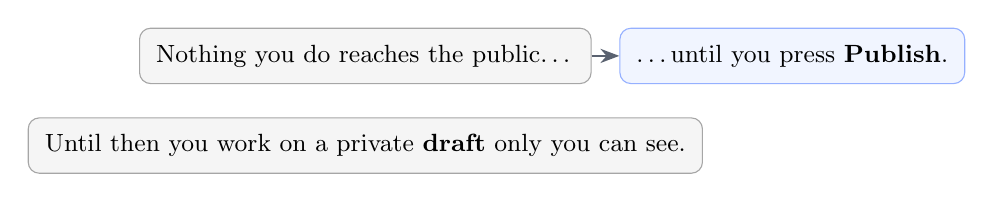
\begin{tikzpicture}[node distance=10pt]
  \node[gbox] (a) {Nothing you do reaches the public\dots};
  \node[box, right=of a] (b) {\dots until you press \textbf{Publish}.};
  \node[gbox, below=12pt of a] (c) {Until then you work on a private \textbf{draft} only you can see.};
  \draw[flow] (a) -- (b);
\end{tikzpicture}

\noindent Read that twice if you are nervous. It is the safety net under everything
below.

% =============================================================================
\section{What the editor \emph{is}}
% =============================================================================

The editor is a thin layer of in-browser software that \textbf{only appears under two
conditions at once}. Understanding those two conditions explains a lot of otherwise
mysterious behaviour.

\paragraph{Condition one: you must be on a \emph{draft} host.} Every Pagesmith site
has at least two addresses. One is the real, public address visitors use (the
\emph{live} or \emph{production} host). The other is a private \emph{draft} host ---
usually \code{localhost} on your own machine, or a quiet preview URL nobody knows.
The editor flatly refuses to load on the live host. This is on purpose: a visitor can
never stumble onto editing controls, and you can never accidentally edit the public
site directly. You edit the draft; the live site changes only when you Publish.

\paragraph{Condition two: you must be signed in as an \emph{editor}.} When you open
the site it checks who you are. A plain visitor just sees the site. If you are signed
in and your account carries the \code{editor} role, a slim toolbar fades in along the
top of the page. That toolbar is the entire editor. There is nothing else to find.

\begin{center}
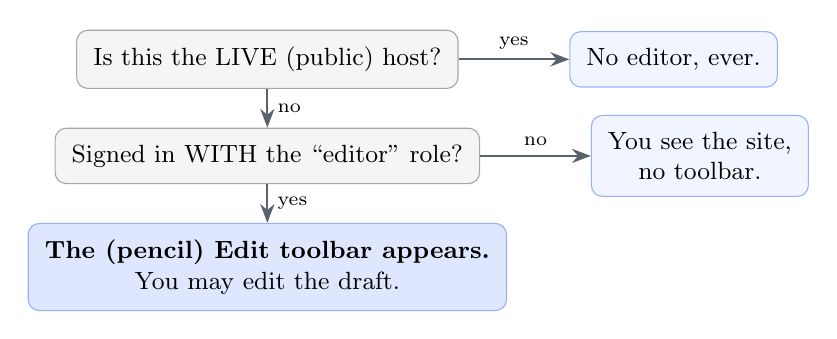
\begin{tikzpicture}[node distance=14pt]
  \node[gbox] (q1) {Is this the LIVE (public) host?};
  \node[box, right=40pt of q1] (no1) {No editor, ever.};
  \node[gbox, below=of q1] (q2) {Signed in WITH the ``editor'' role?};
  \node[box, right=40pt of q2] (no2) {You see the site,\\no toolbar.};
  \node[box, below=of q2, fill=boxblue!18] (yes) {\textbf{The (pencil) Edit toolbar appears.}\\You may edit the draft.};
  \draw[flow] (q1) -- node[above,font=\scriptsize]{yes} (no1);
  \draw[flow] (q1) -- node[right,font=\scriptsize]{no} (q2);
  \draw[flow] (q2) -- node[above,font=\scriptsize]{no} (no2);
  \draw[flow] (q2) -- node[right,font=\scriptsize]{yes} (yes);
\end{tikzpicture}
\end{center}

Why build it this way? To keep the public site \emph{pure}. The code that renders
your live page is exactly the code that renders it for visitors --- the editor is
bolted on top only in the draft world, and leaves no trace on the real one. You never
wonder ``is this an editor thing or a real thing?'' On the live site there are no
editor things.

% =============================================================================
\section{Running it on your own computer}
% =============================================================================

You can run the entire site --- backend and all --- on your own laptop, with no cloud
account and no money spent. This is the safest possible playground: it is a private
draft host by definition, so the editor is available, and nothing reaches the
internet.

\subsection{Prerequisites (install once)}

You need \textbf{Node.js version 20}, plus three command-line tools installed
globally:

\begin{lstlisting}
npm i -g azurite @azure/static-web-apps-cli azure-functions-core-tools@4
\end{lstlisting}

\noindent In plain terms:
\begin{itemize}[leftmargin=*]
  \item \textbf{azurite} --- a tiny local stand-in for cloud storage, so your content
        and images have somewhere to live without a real cloud account.
  \item \textbf{@azure/static-web-apps-cli} (the ``SWA emulator'') --- runs the
        website on your machine exactly the way the cloud would.
  \item \textbf{azure-functions-core-tools@4} --- runs the small backend that saves
        your edits.
\end{itemize}
You install these once and forget about them.

\subsection{Start it}

From the project folder, run one script that does everything --- starts local
storage, fills it with the starter content, and launches the site:

\begin{lstlisting}
./start-local.sh
\end{lstlisting}

\noindent When it finishes, open a browser to:

\begin{lstlisting}
http://localhost:4280
\end{lstlisting}

\subsection{Become an editor}

The first time you open the site, it sends you to a sign-in screen. This is the
emulator's \emph{pretend} login --- it is not asking for a real password. The exact
dance:

\begin{enumerate}[leftmargin=*]
  \item Sign in as the user \code{dev}.
  \item On that same screen, \textbf{add the role \code{editor}} (type \code{editor}
        into the roles field).
  \item Continue.
\end{enumerate}

The page reloads, and now --- because you are on a draft host \emph{and} carry the
\code{editor} role --- the \textbf{(pencil) Edit} toolbar appears across the top. You are in.

\begin{center}
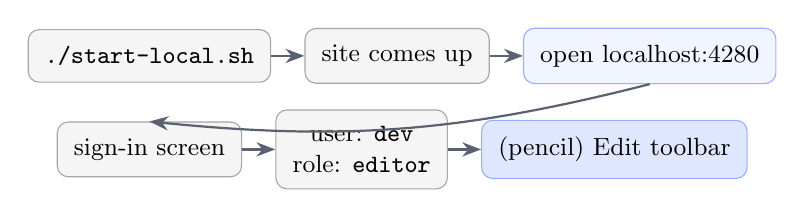
\begin{tikzpicture}[node distance=12pt]
  \node[gbox] (a) {\code{./start-local.sh}};
  \node[gbox, right=of a] (b) {site comes up};
  \node[box, right=of b] (c) {open localhost:4280};
  \node[gbox, below=14pt of a] (d) {sign-in screen};
  \node[gbox, right=of d] (e) {user: \code{dev}\\role: \code{editor}};
  \node[box, right=of e, fill=boxblue!18] (f) {(pencil) Edit toolbar};
  \draw[flow] (a) -- (b); \draw[flow] (b) -- (c);
  \draw[flow] (c.south) to[bend left=10] (d.north);
  \draw[flow] (d) -- (e); \draw[flow] (e) -- (f);
\end{tikzpicture}
\end{center}

\paragraph{If the toolbar doesn't appear} it is almost always the role. Sign out,
sign back in, and make sure you typed \code{editor} (lowercase) into the roles box.
Without that role you are treated as an ordinary visitor --- which is the editor
working exactly as designed.

% =============================================================================
\section{A tour of the toolbar}
% =============================================================================

Everything you can do lives in that one bar at the top.

\begin{center}
\begin{tikzpicture}[font=\scriptsize, node distance=2pt]
  \node[box] (brand) {(rec) wordmark editor};
  \node[box, right=of brand] (ep) {Edit\,/\,Preview};
  \node[box, right=of ep] (pill) {Home};
  \node[box, right=of pill] (sec) {Sections};
  \node[box, right=of sec] (pg) {Pages};
  \node[box, right=of pg] (sv) {Save draft};
  \node[box, right=of sv] (pub) {Publish};
  \node[box, right=of pub] (more) {More $\blacktriangledown$};
  \node[gbox, below=18pt of sec, text width=8.2cm] (menu)
    {\textbf{More $\blacktriangledown$} opens: Theme \textperiodcentered{} Background \textperiodcentered{} Questionnaire \textperiodcentered{} Tracking \textperiodcentered{}
     Responses \textperiodcentered{} Refresh stats \textperiodcentered{} Revert \textperiodcentered{} Help \textperiodcentered{} Log out};
  \draw[flow] (more.south) to[bend left=15] (menu.east);
\end{tikzpicture}
\end{center}

One short paragraph each. You need not memorise these; just know they exist.

\begin{description}[style=nextline,leftmargin=1.4em]
  \item[The brand corner] A small recording-style dot, your site's wordmark, and the
    word ``editor''. The dot is a gentle ``rec'' light reminding you that changes here
    are a private \emph{draft}, not live. Decoration, not a button.
  \item[Edit / Preview] The master switch. \textbf{Edit} turns on the editing layer
    (a dashed outline appears around everything you can change). \textbf{Preview}
    hides every control so you see the page exactly as a visitor would. Toggling saves
    or discards nothing --- it just shows or hides the controls.
  \item[The page pill] Shows which page you are editing (e.g.\ ``Home'') and its state:
    ``Home --- draft'' normally, ``Home --- unsaved'' when you have unsaved changes. A
    handy ``do I have unsaved work?'' indicator.
  \item[Sections] Opens the \textbf{Sections panel} to add, hide, delete, and reorder
    the building blocks of the current page. Important --- and it has one quirk, in
    Section~\ref{sec:sections}.
  \item[Pages] Opens the \textbf{Pages panel}: create pages and set each page's
    visibility. See Section~\ref{sec:pages}.
  \item[Save draft] Saves everything you changed to your private draft. Only you can
    see a draft. Press it often and without fear --- it makes nothing public.
  \item[Publish] The one button that reaches the world: it copies your saved draft
    onto the live site. Habit: Save, look, \emph{then} Publish.
  \item[More $\blacktriangledown$] A dropdown holding the less-frequent tools (Theme, Background,
    Questionnaire, Tracking, Responses, Refresh stats, Revert, Help, Log out), so the
    bar stays tidy.
\end{description}

\noindent The \textbf{More $\blacktriangledown$} entries, briefly: \textbf{Theme} (site-wide colours),
\textbf{Background} (the big page background image), \textbf{Questionnaire} (edit the
signup-survey questions), \textbf{Tracking} (paste analytics IDs), \textbf{Responses}
(download submitted answers), \textbf{Refresh stats} (pull live numbers where wired
up --- safe to ignore otherwise), \textbf{Revert} (throw away all unpublished changes
and snap back to live), \textbf{Help} (built-in help), \textbf{Log out}.

% =============================================================================
\section{Editing the content that's already there}\label{sec:inline}
% =============================================================================

This is the part that feels like magic the first time. With \textbf{Edit} on, you
change things by clicking the actual thing on the page.

\paragraph{Text: click it and type.} Click a headline, a paragraph, a button label
--- any text with the dashed outline --- and a cursor appears right inside it. Type.
Backspace. It behaves like a text box, except the ``text box'' \emph{is} the headline
on your page, sized and styled exactly as it will look published. Click away when
done. Each edit is written into the draft as you type, and the page pill flips to
``--- unsaved'' to remind you to \textbf{Save draft} before you leave. Until you Save,
changes live only in this browser tab; reloading throws them away (that is the safety
net, not a bug).

\paragraph{A small honesty note about pasting.} Typing plain text is perfect. If you
\emph{paste} text copied from Word or a web page, the browser sometimes smuggles in
invisible formatting. For the cleanest result, paste as plain text (often
Ctrl/Cmd-Shift-V) or just type. Nothing breaks if you don't --- it is only tidier.

\paragraph{Images: click to open the media picker.} Click an image and the
\textbf{media picker} opens --- a little gallery of pictures already in your site,
organised into folders (tabs). You can \emph{choose an existing image} (click a
thumbnail) or \emph{upload a new one} (pick a file; it is added to the library and
selected). Pick one and the image swaps immediately. Uploads are optimised
automatically so pages stay fast; you need not think about it.

\paragraph{Per-element text styling.} Sometimes you want \emph{this one} heading
bigger, or \emph{this one} paragraph centred, without touching the rest of the site.
You reach that through the section's \textbf{Edit} panel (next section), which offers
small controls for alignment (Left / Center / Right), text colour, and size on the
individual pieces of text. Leave a styling field blank and that element inherits the
site-wide look --- so \textbf{blank means ``use the default'', not ``make it blank''.}
That gentle rule holds throughout the editor.

% =============================================================================
\section{The Sections panel --- and the one big gotcha}\label{sec:sections}
% =============================================================================

A page is built from \textbf{sections} stacked top to bottom: a headline, a gallery,
a block of text, a video. The \textbf{Sections} button opens the panel that manages
them. Each section gets a row with a few controls:

\begin{lstlisting}
  +-------------------------------------------------------------------+
  |  drag   Heading: "Welcome"       [Hide] [View] [Edit] [Delete]    |
  |  drag   Photo gallery (8)        [Hide] [View] [Edit] [Delete]    |
  |  drag   Text: "About us"         [Hide] [View] [Edit] [Delete]    |
  |                                                                   |
  |  + Add section                                                    |
  |                                                                   |
  |  Across the whole site                                            |
  |     Header / nav                       [View] [Edit]              |
  |     Footer                             [View] [Edit]              |
  |                                                                   |
  |            [ Cancel ]            [ Apply & Save ]                 |
  +-------------------------------------------------------------------+
\end{lstlisting}

\begin{description}[style=nextline,leftmargin=1.4em]
  \item[drag] Grab here to reorder (Section~\ref{sec:reorder}).
  \item[Hide] Takes a section off the page but keeps it in the list, so you can
    \textbf{Show} it again later --- perfect for something seasonal you will want back.
    Nothing is lost.
  \item[View] Jumps the page to that section so you can see what you are working on.
  \item[Edit] Opens that section's content (its text, images, list of items).
  \item[Delete] Removes an \emph{added} section. A little \textbf{Undo} appears right
    after, in case it was a mistake.
\end{description}

\noindent The site-wide rows (``Across the whole site'' --- header/nav and footer)
offer only \textbf{View} and \textbf{Edit}, because they appear on every page.

\subsection{Now, the gotcha. Read this slowly.}

\textbf{The Sections panel is a \emph{staging} editor.} When you Hide, Delete,
reorder, or Add here, \emph{the live page underneath does not change as you click.}
Your clicks are collected --- like a shopping list --- and nothing happens to the
page until you press \textbf{Apply \& Save}. Press \textbf{Cancel} and the list is
forgotten; the page is untouched.

This trips people up because the rest of the editor is so immediate. Here, on purpose,
it is not. Why? Because reordering and deleting whole sections are big structural
moves, and it is safer to plan them all and apply them in one deliberate step than to
have the page leaping around under your cursor.

\begin{center}
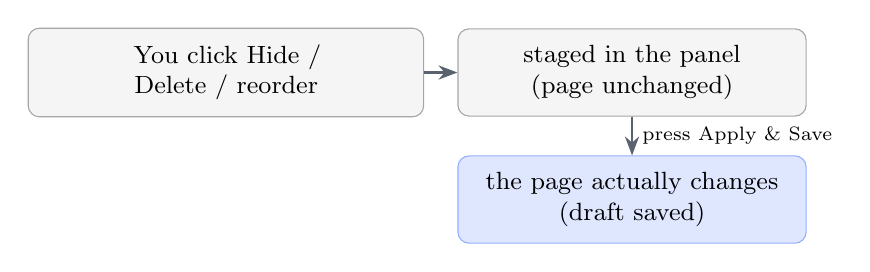
\begin{tikzpicture}[node distance=12pt]
  \node[gbox, text width=4.6cm] (a) {You click Hide / Delete / reorder};
  \node[gbox, right=of a, text width=4.0cm] (b) {staged in the panel\\(page unchanged)};
  \node[box, below=14pt of b, fill=boxblue!18, text width=4.0cm] (c) {the page actually changes\\(draft saved)};
  \draw[flow] (a) -- (b);
  \draw[flow] (b) -- node[right,font=\scriptsize]{press Apply \& Save} (c);
\end{tikzpicture}
\end{center}

So if you Delete a section and the page still shows it --- that is correct. It goes
when you Apply \& Save. And \textbf{Delete has an Undo right up until you save}: undo
it in the panel and it is as if you never touched it. Even once saved to your draft,
nothing is \emph{public} until you Publish, and \textbf{Revert} can still rescue you.

\paragraph{The two-word rule of thumb.} \emph{Hide} means ``not now, maybe later'' ---
reversible any time, forever. \emph{Delete} means ``gone'' --- but only undoable until
you save. When in doubt, Hide.

% =============================================================================
\section{Adding a new section}
% =============================================================================

Inside the Sections panel, click \textbf{+ Add section}. This opens the \textbf{parts
library} --- a grid of tiles, one per kind of section: Text, Heading, Photo gallery,
Video, Carousel, Links, and more, each with a little preview.

\begin{center}
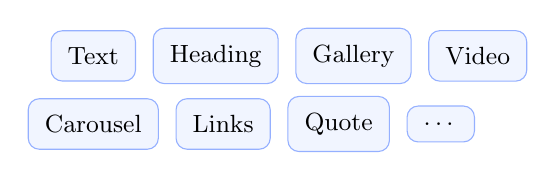
\begin{tikzpicture}[font=\scriptsize, node distance=6pt]
  \node[box] (t1) {Text};   \node[box, right=of t1] (t2) {Heading};
  \node[box, right=of t2] (t3) {Gallery}; \node[box, right=of t3] (t4) {Video};
  \node[box, below=of t1] (t5) {Carousel}; \node[box, right=of t5] (t6) {Links};
  \node[box, right=of t6] (t7) {Quote}; \node[box, right=of t7] (t8) {\dots};
\end{tikzpicture}
\end{center}

Click a tile and that part \textbf{drops into your page pre-filled} with placeholder
content --- a sample heading, a couple of example items. You never face a scary blank
box. From there you edit it like anything else: click the placeholder text to replace
it, click an image to swap it.

\paragraph{The tiles are clickable cards, not buttons} --- so just click anywhere on
the tile. (We mention this only because people occasionally go hunting for a button to
press.)

\subsection{Lists inside a section (galleries, links, \dots)}

Some sections are not a single thing --- they are a \emph{list} of things: a gallery
is a list of images, a ``links'' block a list of links, a carousel a list of slides.
You \textbf{edit those lists from the section's Edit panel}, not by hovering on the
page. Open the section's \textbf{Edit} and you will see a button like \textbf{``Edit
gallery (8)''} or \textbf{``Edit links (3)''} --- the number tells you how many items
are in there. Click it to add items, fill in each one's fields (text, a URL, an
image), and reorder them.

This is deliberate: a single, predictable place to manage a list rather than a scatter
of hover controls. So if you ever think ``where did the images go, I can't find them''
--- they are behind the section's \textbf{Edit $\rightarrow$ Edit gallery (N)}.

% =============================================================================
\section{Reordering things}\label{sec:reorder}
% =============================================================================

Two ways, depending on what you move.

\paragraph{Sections on a page.} In the Sections panel, grab a row by its drag handle
and drag it up or down. (Remember: staged --- press \textbf{Apply \& Save} to make it
real.) You can also drag a list \emph{item} directly on the page: hover over an item,
a small grip appears, drag it.

\paragraph{Items inside a Group.} Some parts are ``Groups'' --- a section holding a few
sub-items side by side. Inside a Group you will find small \textbf{Up\,/\,Down}
controls on each item to nudge it one step at a time, often easier than dragging when
things are close together.

% =============================================================================
\section{Theme \& Background}
% =============================================================================

These live in the \textbf{More $\blacktriangledown$} menu and control how the site \emph{looks} rather
than what it \emph{says}.

\subsection{Theme --- site-wide colours}

\textbf{Theme} opens a colour panel. Change the main accent colour (buttons, links,
highlights) and a couple of others, and the whole site shifts to match. There is also
a palette used by chart-like and decorative parts. Theme changes are
\textbf{site-wide} --- they affect every page. To restyle \emph{just one section},
don't use Theme; use that section's own styling (via its \textbf{Edit} panel,
Section~\ref{sec:inline}). The rule: Theme = everything; section styling = this one
section.

\paragraph{A small known wrinkle.} If you \emph{clear} one of the three primary theme
colours hoping it falls back to the built-in default, the live page may keep showing
the old colour until you reload. Reloading sorts it out. (Setting a \emph{new} colour
always works immediately; only the ``clear back to default'' case needs a refresh.)

\subsection{Background --- the big image behind a page}

\textbf{Background} sets the large image behind the page content. It opens the same
media picker --- choose an existing image or upload a new one. You can set a different
image for \textbf{large screens (desktop/tablet)} and for \textbf{phones}, so the
background looks right on both.

\paragraph{} If you upload a new background but \emph{reuse a filename}, your browser
may show the old cached version. A hard refresh (Ctrl/Cmd-Shift-R) forces it to fetch
the new one. The editor will even hint this to you when it happens.

% =============================================================================
\section{Pages and the three visibility levels}\label{sec:pages}
% =============================================================================

The \textbf{Pages} button opens the Pages panel, where you create pages and decide
who can reach them.

\paragraph{Creating a page.} Type a name (e.g.\ ``Press'') and create it. The new page
starts empty --- open it and build it up from the parts library like any other page.
No code, no setup; a fresh page works at its own URL the moment you save it.

\paragraph{Visibility.} Every page has one of three levels, and each means something
specific for your \emph{live} site:

\begin{center}
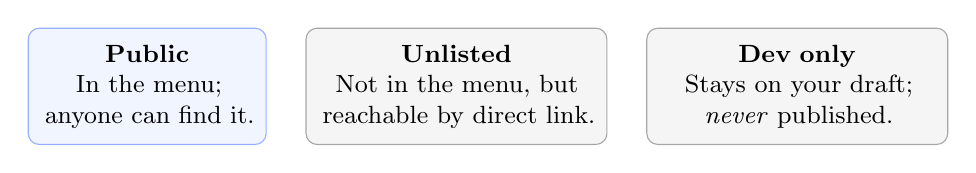
\begin{tikzpicture}[font=\small, node distance=8pt]
  \node[box, text width=2.6cm] (pub) {\textbf{Public}\\In the menu;\\anyone can find it.};
  \node[gbox, right=14pt of pub, text width=3.4cm] (unl) {\textbf{Unlisted}\\Not in the menu, but\\reachable by direct link.};
  \node[gbox, right=14pt of unl, text width=3.4cm] (dev) {\textbf{Dev only}\\Stays on your draft;\\\emph{never} published.};
\end{tikzpicture}
\end{center}

\begin{itemize}[leftmargin=*]
  \item \textbf{Public} --- the normal case. The page appears in your navigation menu
    and anyone can find it. Most pages are Public.
  \item \textbf{Unlisted} --- not in the menu, but anyone you give the link to can open
    it. Ideal for a press kit or a page you share directly rather than advertise.
  \item \textbf{Dev only} --- stays on your private draft and is \textbf{never
    published}. Use it for works-in-progress and admin-only pages. When you Publish,
    Dev-only pages are skipped automatically --- they simply don't exist on the public
    site.
\end{itemize}

New pages start as Public; set them Unlisted or Dev only if they are not ready. You
can change a page's visibility any time, and the change is saved as soon as you pick
it.

% =============================================================================
\section{The signup survey: Questionnaire \& Responses}
% =============================================================================

Pagesmith includes a built-in signup flow --- a way for visitors to give you their
email and answer a few questions. Two tools in \textbf{More $\blacktriangledown$} run it:
\textbf{Questionnaire} (edit the questions) and \textbf{Responses} (download the
answers). The visitor's experience flows like this:

\begin{center}
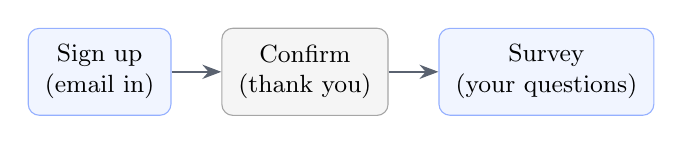
\begin{tikzpicture}[node distance=18pt]
  \node[box] (s) {Sign up\\(email in)};
  \node[gbox, right=of s] (c) {Confirm\\(thank you)};
  \node[box, right=of c] (q) {Survey\\(your questions)};
  \draw[flow] (s) -- (c); \draw[flow] (c) -- (q);
\end{tikzpicture}
\end{center}

\subsection{Editing the questions (Questionnaire)}

Open \textbf{Questionnaire} to edit the intro text and the list of questions. Use
\textbf{Edit questions} to add, remove, and reorder them. A few honest details:

\begin{itemize}[leftmargin=*]
  \item \textbf{A question with a blank label is skipped entirely.} So ``an empty
    question box'' means ``no question here'', not ``a blank question''. To remove a
    question, you can clear it.
  \item The \textbf{email box is always present} --- the core of a signup; you need not
    add it.
  \item \textbf{Renaming a question keeps its answers lined up.} Each question becomes
    a \emph{column} in the downloaded responses; renaming doesn't scramble answers
    already given, and removing a question doesn't touch answers already submitted.
\end{itemize}

\subsection{Where responses go (Responses)}

Click \textbf{Responses} and the submitted answers download to your computer as a file
(CSV --- the kind a spreadsheet opens; a JSON option is available too). Each question
is a column, each submission a row. That is the whole loop: you set the questions here,
visitors answer on the live site, and you collect the results with one click.

% =============================================================================
\section{Tracking (analytics \& pixels)}
% =============================================================================

To measure traffic --- with Google Analytics, a Meta (Facebook) Pixel, or similar ---
open \textbf{Tracking} from \textbf{More $\blacktriangledown$} and paste in your IDs. There is a field for
each; paste, save, done. Entirely optional; the site works perfectly without it.

\paragraph{One important rule.} Tracking only fires on the \textbf{live} site. It
deliberately does \emph{not} run on your draft host --- a feature, because it means
your own editing and testing never pollute your real analytics with fake visits. So
don't be alarmed if you paste a tracking ID and see no activity while editing locally;
it switches on once the page is published and a real visitor loads it.

% =============================================================================
\section{Saving \& publishing --- the mental model}
% =============================================================================

This is the most important section to internalise, and it is simple once it clicks.
There are two copies of your site: a private \textbf{draft} and the public
\textbf{live} site. Three buttons move things between them.

\begin{center}
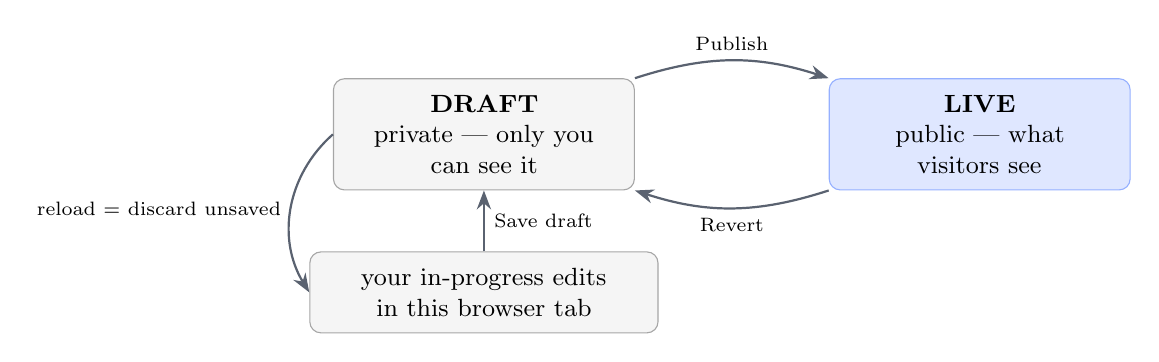
\begin{tikzpicture}[node distance=26pt]
  \node[gbox, text width=3.4cm] (draft) {\textbf{DRAFT}\\private --- only you\\can see it};
  \node[box, right=70pt of draft, text width=3.4cm, fill=boxblue!18] (live) {\textbf{LIVE}\\public --- what\\visitors see};
  \node[gbox, below=22pt of draft, text width=4.0cm] (edits) {your in-progress edits\\in this browser tab};
  \draw[flow] (draft.north east) to[bend left=18] node[above,font=\scriptsize]{Publish} (live.north west);
  \draw[flow] (live.south west) to[bend left=18] node[below,font=\scriptsize]{Revert} (draft.south east);
  \draw[flow] (edits.north) -- node[right,font=\scriptsize]{Save draft} (draft.south);
  \draw[flow] (draft.west) to[bend right=40] node[left,font=\scriptsize]{reload = discard unsaved} (edits.west);
\end{tikzpicture}
\end{center}

\begin{description}[style=nextline,leftmargin=1.4em]
  \item[Save draft] Write your current edits into the private draft. Now they are
    safely stored (they survive a reload), but still private. Press this often.
  \item[Publish] Copy the saved draft onto the live, public site. \emph{The only step
    visitors ever see.} Publish takes your last \emph{saved} draft --- so the reliable
    habit is \textbf{Save $\rightarrow$ look it over $\rightarrow$ Publish}.
  \item[Revert] Discard every unpublished change and restore whatever is currently
    live. Your big ``undo everything since the last Publish'' rescue button. (Dev-only
    pages are never published, so Publish skips them automatically.)
\end{description}

\paragraph{One thing that surprises people: some panels reload the page after you
save.} When you finish in certain panels (a list editor, the Theme panel, adding a
section), the page refreshes itself to redraw cleanly. This is completely normal and
expected --- not an error, and you lost nothing; your save already happened. Just let
it settle.

And the safety net, once more: until you press \textbf{Publish}, the public sees
nothing. Until you press \textbf{Save draft}, even your draft doesn't have it --- a
reload returns you to the last saved state. Between those two facts, it is very hard to
do real damage.

% =============================================================================
\section{The ``?'' help buttons}
% =============================================================================

You need not keep this guide open while you work. \textbf{Next to the heading of
almost every panel there is a small round ``?'' button.} Click it and a short,
plain-language note opens, written for exactly the panel you are in --- what the
buttons do, what happens if you leave a field blank, the little edge cases. There is
also a general \textbf{Help} entry in \textbf{More $\blacktriangledown$} for the overview.

These notes are deliberately honest about the fiddly bits (the same edge cases this
guide calls out --- blank questions skipped, ``empty means inherit'', the
cache-refresh quirk). So when you are mid-task and wondering ``wait, what does
\emph{this} do?'', the answer is one click away, right where you are.

% =============================================================================
\section{Your first edit (a 60-second tutorial)}
% =============================================================================

Let's prove the whole loop works, end to end, with the smallest possible change:
editing the home page headline and watching it persist.

\begin{lstlisting}
  1. Turn on editing     ->  click [Edit] in the toolbar.
                             verify: a dashed outline appears around editable things.

  2. Find the headline   ->  scroll to the big headline on the Home page.
                             verify: hovering it shows the dashed outline.

  3. Change it           ->  click the headline, select the text, type something new.
                             verify: the page shows your new words, and the page pill
                                     reads "Home - unsaved".

  4. Save it             ->  click [Save draft].
                             verify: the pill changes back to "Home - draft".

  5. Prove it persisted  ->  reload the browser (F5 / Cmd-R).
                             verify: your new headline is STILL there.
                                     (Had you skipped step 4, the reload would have
                                      brought back the old headline - the safety net
                                      doing its job.)
\end{lstlisting}

That is the entire rhythm of working in Pagesmith, in miniature: \textbf{Edit
$\rightarrow$ change $\rightarrow$ Save $\rightarrow$ it sticks.} Everything else in
this guide is just more \emph{kinds} of change (images, sections, pages, colours) hung
on that same simple loop. When you are ready to share your work with the world, you do
it one more way --- \textbf{Publish} --- and your saved draft becomes the live site.

\bigskip
\noindent Welcome aboard. Go make something.

\end{document}
